%% =============================================================
%%  Les mordants — du signe aux notes jouées
%%  Guide de référence, composé en LaTeX, gravures LilyPond
%% =============================================================
%%
%%  Les figures (gravures/m-*.cropped.pdf), les réponses de l'exercice
%%  (gravures/mordants-reponses.tex) et le fichier mordants.musicxml
%%  sont produits par outils/generer_mordants.py, à partir du modèle
%%  de hauteurs des autres guides (outils/gammes.py). Voir le colophon
%%  en dernière page.
%%
\documentclass[a4paper,11pt]{article}

\usepackage[top=2.2cm,bottom=2.4cm,left=2.2cm,right=2.2cm]{geometry}
\usepackage[T1]{fontenc}
\usepackage[utf8]{inputenc}
\usepackage[french]{babel}
\usepackage{lmodern}
\usepackage{xcolor}
\usepackage{graphicx}
\usepackage{titlesec}
\usepackage{fancyhdr}
\usepackage{mdframed}
\usepackage{enumitem}
\usepackage{hyperref}

\graphicspath{{gravures/}}

% ---- Couleurs, reprises du document des accords de guitare ---------
\definecolor{navy}{RGB}{18,50,105}
\definecolor{lightnavy}{RGB}{235,241,255}
\definecolor{mygray}{RGB}{110,110,110}

\hypersetup{colorlinks=true, linkcolor=navy, urlcolor=navy,
  pdftitle={Les mordants — du signe aux notes jouées},
  pdfauthor={Fabian Bastin}}

% ---- En-tête et pied -----------------------------------------------
\pagestyle{fancy}
\fancyhf{}
\renewcommand{\headrulewidth}{0.4pt}
\renewcommand{\footrulewidth}{0.4pt}
\fancyhead[L]{\small\bfseries\textcolor{navy}{Les mordants}}
\fancyhead[R]{\small\textcolor{mygray}{\thepage}}
\fancyfoot[C]{\small\textcolor{mygray}{Du signe aux notes jouées}}

% ---- Titres de section ---------------------------------------------
\newcommand{\navysect}[1]{%
  \colorbox{navy}{%
    \parbox[c][17pt]{\dimexpr\linewidth-2\fboxsep\relax}{%
      \color{white}\hspace{6pt}\bfseries\normalsize #1}}%
}
\titleformat{\section}[block]{\normalfont}{}{0pt}{\navysect}
\titlespacing*{\section}{0pt}{16pt}{10pt}

% ---- Encadré de remarque -------------------------------------------
\newmdenv[linecolor=navy, linewidth=0.5pt, backgroundcolor=lightnavy,
  innertopmargin=6pt, innerbottommargin=6pt,
  innerleftmargin=8pt, innerrightmargin=8pt,
  skipabove=8pt, skipbelow=8pt]{remarque}

% ---- Figure gravée ---------------------------------------------------
% Figure gravée, à la largeur donnée (part de la ligne), avec sa légende.
% Le tout tient dans une minipage : figure et légende ne sont jamais
% séparées par un saut de page.
\newcommand{\gravure}[3]{%
  \par\medskip\noindent
  \begin{minipage}{\linewidth}
    \centering
    \includegraphics[width=#2\linewidth]{#1.cropped.pdf}\\[4pt]
    {\small\itshape\color{mygray} #3}
  \end{minipage}\par\medskip
}

\setlist{itemsep=2pt, topsep=4pt, parsep=0pt}

\begin{document}

% =====================================================================
\begin{titlepage}
\centering
\vspace*{3cm}
{\Huge\bfseries\color{navy} Les mordants\par}
\vspace{0.6cm}
{\LARGE\color{navy} Du signe aux notes jouées\par}
\vspace{1.4cm}
{\large Une note, sa voisine, la note\par}
\vspace{2.5cm}
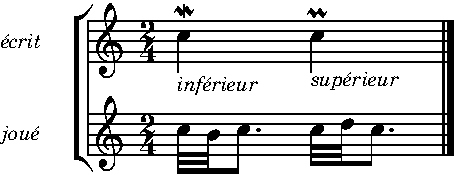
\includegraphics[width=0.6\linewidth]{m-deux.cropped.pdf}
\vfill
{\small\color{mygray}
Gravures LilyPond, composition \LaTeX.\\
Fichier MusicXML joint.\par}
\vspace{1cm}
\end{titlepage}

\tableofcontents
\newpage

% =====================================================================
\section{Avant-propos}

Un \textbf{mordant} est un ornement bref : la note écrite, une note voisine,
puis de nouveau la note, les deux premières très vite, la dernière tenue. Il y
en a deux, selon le côté de la voisine : le \emph{mordant inférieur} descend
vers la voisine du dessous, le \emph{mordant supérieur} monte vers celle du
dessus. Le nom vient de l'italien \emph{mordente}, du latin \emph{mordere},
mordre : l'ornement mord la note et la lâche aussitôt. Le \emph{trille}, qui
alterne la note et sa voisine du dessus jusqu'au bout de la valeur, en est le
proche parent. Au programme de matières théoriques de l'École de musique
Vincent-d'Indy, ces notions relèvent des niveaux 3 et 5 ;
\href{https://www.slashbin.net/musique/theorie/ornements.pdf}{\emph{Les
ornements}} présentent les autres, de l'appogiature au gruppetto.

À lire après
\href{https://www.slashbin.net/musique/theorie/lecture.pdf}{\emph{Lire les
notes}} et
\href{https://www.slashbin.net/musique/theorie/intervalles.pdf}{\emph{Les
intervalles}} : les exemples sont en clé de sol, et l'écart entre une note et
sa voisine s'y mesure en tons et en demi-tons. Cette voisine se prend dans la
gamme que désigne l'armure, dont traitent
\href{https://www.slashbin.net/musique/theorie/gammes.pdf}{\emph{Les
gammes}}.

\begin{remarque}
\textbf{Conventions.} Les notes sont nommées en français. La \emph{note
principale} est la note écrite ; sa \emph{voisine}, ou note auxiliaire, la note
immédiatement au-dessus ou au-dessous dans la gamme. Les exemples sont en clé de
sol et, sauf mention contraire, en do majeur. Les notes jouées y sont écrites
en triples croches, l'allure d'un mordant à la noire 80 : un peu moins d'un
dixième de seconde par note.
\end{remarque}

Le fichier MusicXML joint fait entendre chaque exemple ; la
section~\ref{sec:musicxml} le présente.

% =====================================================================
\section{Deux mordants}
\label{sec:signe}

\textbf{Deux signes.} Le mordant s'écrit par un court zigzag au-dessus de la
note. Barré d'un trait vertical, c'est le \textbf{mordant inférieur} : la
note, sa voisine du dessous, la note. Sans trait, c'est le \textbf{mordant
supérieur} : la note, sa voisine du dessus, la note.

\gravure{m-deux}{0.54}{Le mordant inférieur, puis le mordant supérieur, sur
do : do, si, do ; puis do, ré, do.}

\textbf{Les trois notes.} Dans les deux cas, les deux premières notes passent
vite, la troisième est tenue jusqu'au bout de la valeur. L'ornement ne quitte
la note que d'un degré, une seule fois, et y revient : on entend la note
elle-même, à peine troublée à son début.

\textbf{La voisine se prend dans la gamme.} Celle du dessous porte le nom qui
précède celui de la note : si sous do, do sous ré. Selon la place de la note
dans la gamme, elle est à un ton ou à un demi-ton --- en do majeur, si est à
un demi-ton sous do, do à un ton sous ré. Dans les deux cas, la note et sa
voisine forment une seconde, mineure ou majeure.

\gravure{m-inferieur}{0.85}{Le mordant inférieur sur do, ré, mi et fa, en do
majeur : écrit en haut, joué en bas. La voisine est à un demi-ton sous do et
fa, à un ton sous ré et mi.}

\textbf{Au-dessus, de même.} La voisine du dessus porte le nom qui suit : ré
sur do, fa sur mi. En do majeur, elle n'est à un demi-ton qu'au-dessus de mi et
de si.

\gravure{m-superieur}{0.85}{Le mordant supérieur sur do, ré, mi et fa : la
voisine est à un ton au-dessus de do, ré et fa, à un demi-ton au-dessus de mi.}

% =====================================================================
\section{Le temps du mordant}
\label{sec:temps}

\textbf{Sur le temps.} Le mordant, inférieur ou supérieur, commence sur la note
écrite, au moment où elle tombe : il prend son temps sur elle, non sur la note
qui précède. Dans les gravures, chaque groupe joué commence exactement sous la
note écrite.

\textbf{Vite, quelle que soit la valeur.} Sur une blanche comme sur une
croche, la note et sa voisine passent aussi vite ; c'est la note tenue qui
s'allonge ou se raccourcit. Joué lentement, le mordant ne mordrait plus : ce
serait un motif de trois notes.

\gravure{m-valeurs}{0.76}{Le même mordant inférieur sur une blanche, une noire
et une croche : deux triples croches chaque fois, la note principale garde le
reste.}

\textbf{L'allure suit le tempo.} Les triples croches des exemples sont une
commodité d'écriture. Dans un mouvement lent, le mordant reste vif et la note
tenue s'allonge ; dans un mouvement rapide, il se resserre jusqu'à n'être plus
qu'un frémissement au début de la note.

\textbf{Le mordant inférieur chez C.~P.~E. Bach.} Dans son \emph{Essai sur la
vraie manière de jouer des instruments à clavier} (1753), il le place de
préférence sur une note qui monte, par degré ou par saut, et jamais sur une
seconde descendante. Il s'en sert pour remplir une note longue --- liée,
pointée, syncopée --- et pour faire briller des notes détachées ou prises par
saut. Dans la basse, ajoute-t-il, c'est l'ornement le plus fréquent, même là
où rien ne l'indique.

% =====================================================================
\section{La voisine et les altérations}
\label{sec:alterations}

\textbf{L'armure d'abord.} Sans autre indication, la voisine prend
l'altération que lui donne l'armure. Sous sol, c'est fa en do majeur, à un
ton ; fa dièse en sol majeur, à un demi-ton.

\textbf{Une altération près du signe.} Pour changer la voisine, on écrit une
petite altération près du signe, du côté de cette voisine : au-dessous pour le
mordant inférieur, au-dessus pour le mordant supérieur. Elle ne touche que la
voisine de cet ornement : la note écrite garde son altération.

\gravure{m-alterations}{0.85}{Sol orné d'un mordant inférieur : en do majeur,
avec un dièse sous le signe, puis en sol majeur. Le dièse écrit et l'armure
donnent la même voisine, fa dièse.}

\textbf{Le demi-ton baroque.} Dans la musique baroque, la voisine inférieure
se prend volontiers à un demi-ton, qui mord davantage : C.~P.~E. Bach note
qu'elle reçoit souvent une altération qui la hausse. Quand le signe n'en porte
pas, l'interprète en juge selon l'harmonie.

% =====================================================================
\section{Les noms des mordants}
\label{sec:superieur}

\textbf{Le mordant inférieur.} L'allemand l'appelle \emph{Mordent}, l'anglais
\emph{lower mordent}, ou \emph{mordent} tout court ; les clavecinistes
français disaient \emph{pincé} (section~\ref{sec:long}).

\textbf{Le mordant supérieur.} L'allemand l'appelle \emph{Pralltriller}, le
trille qui rebondit, ou \emph{Schneller}. L'anglais l'appelle aujourd'hui
\emph{upper} ou \emph{inverted mordent}, mais au XIX\textsuperscript{e}
siècle, \emph{mordent} y désignait souvent le mordant supérieur, et
\emph{inverted mordent} l'inférieur.

\begin{remarque}
\textbf{Le trait ne trompe pas.} Les noms changent d'une langue et d'une époque
à l'autre ; barré, le signe désigne toujours la voisine du dessous. C'est le
zigzag sans trait dont le sens a changé (section~\ref{sec:epoques}).
\end{remarque}

% =====================================================================
\section{Le mordant long}
\label{sec:long}

Un zigzag plus long, toujours barré, double l'alternance du mordant
inférieur : la note, sa voisine du dessous, la note, sa voisine, la note.
Couperin distingue ainsi un \emph{pincé simple} et un \emph{pincé double}, plus
long. C.~P.~E. Bach distingue de même un mordant court et un mordant long ; le
signe du long ne s'allonge jamais davantage, mais son exécution peut compter
plus d'alternances, pour remplir une note longue.

\gravure{m-long}{0.6}{Le mordant inférieur, puis le mordant long, chacun sur
une noire : trois notes, puis cinq.}

% =====================================================================
\section{Le trille}
\label{sec:trille}

\textbf{Une alternance.} Le \textbf{trille} alterne rapidement la note écrite
et sa voisine du dessus, prise dans la gamme, à un ton ou à un demi-ton, et
cela jusqu'au bout de la valeur. Il s'écrit \emph{tr} au-dessus de la note,
seul ou suivi d'une ligne ondulée qui en marque la durée. Entre deux notes plus
éloignées qu'un ton, l'alternance rapide ne s'appelle plus trille, mais
\emph{trémolo} (\emph{Les ornements}).

\textbf{Du mordant au trille.} Le mordant supérieur sonne comme le début d'un
trille commencé sur la note : do, ré, do. Le mordant s'arrête là et tient la
note ; le trille continue d'alterner.

\textbf{Le trille altéré.} Comme pour le mordant, une petite altération près
du \emph{tr} change la voisine. Sur ré, en do majeur, le trille alterne avec mi,
à un ton ; avec un bémol près du signe, avec mi bémol, à un demi-ton.

\gravure{m-trille-debut}{1}{Sur do, le mordant supérieur, puis le trille
commencé sur la note : les mêmes trois premières notes. Sur ré, le trille
alterne avec mi ; avec le bémol, avec mi bémol.}

\textbf{La vitesse.} Elle ne se compte pas en notes : elle dépend du tempo et
du caractère. Un trille très rapide dans un mouvement lent paraît nerveux, un
trille lent dans un mouvement vif paraît lourd. Sur une note longue,
l'interprète peut le commencer posément et l'accélérer. Les gravures, faute de
mieux, l'écrivent en triples croches, huit par noire à la noire 80.

\textbf{La note de départ.} À l'époque baroque, le trille commence par le haut,
sur la voisine, et sur le temps : c'est ainsi que le note la table d'ornements
de Bach (section~\ref{sec:epoques}), et C.~P.~E. Bach en fait la règle. Au
XIX\textsuperscript{e} siècle, il commence le plus souvent sur la note
elle-même ; la méthode de piano de Hummel, en 1828, ne donne plus que cette
manière. Entre les deux, et d'un compositeur ou d'une édition à l'autre,
l'usage varie : le contexte et le style décident. Une petite note écrite
devant le trille lève le doute, puisqu'elle en donne la première note.

\textbf{La terminaison.} Un trille sur une note longue s'achève souvent par
deux petites notes écrites après lui : la voisine du dessous, puis la note,
qui mènent à la note suivante.

\gravure{m-trille}{0.96}{Un trille long sur ré, avec la ligne ondulée et la
terminaison, do et ré, puis do : au XVIII\textsuperscript{e} siècle, commencé
sur la voisine, mi ; au XIX\textsuperscript{e}, sur la note. Dans les deux
cas, la terminaison le conclut.}

\textbf{Mordant, trille, gruppetto.} Trois ornements tournent autour d'une
note. Le mordant la quitte une fois, d'un côté, et y revient ; elle est ensuite
tenue. Le trille alterne avec la voisine du dessus jusqu'au bout de la valeur.
Le \emph{gruppetto} en fait le tour : la voisine du dessus, la note, la voisine
du dessous, la note. Le mordant est le plus bref des trois : il orne le début
de la note sans en changer le caractère, là où le trille la fait vibrer d'un
bout à l'autre.

\gravure{m-voisins}{0.87}{Le mordant inférieur, le trille et le gruppetto sur
une même note. Le trille commence ici sur la note, comme depuis le
XIX\textsuperscript{e} siècle.}

% =====================================================================
\section{Un signe, deux lectures}
\label{sec:epoques}

\textbf{Chez Bach.} En 1720, Jean-Sébastien Bach écrit pour son fils
Wilhelm Friedemann une table des ornements. Le zigzag barré y porte le nom de
\emph{Mordant} et se joue comme le mordant inférieur d'aujourd'hui : la note,
sa voisine du dessous, la note. Le zigzag sans trait, lui, y est un
\emph{trille} (\emph{Trillo}) : il commence sur la voisine du dessus et
alterne avec la note. Sur une note brève, on le réduit à quatre notes, la
dernière tenue.

\textbf{Chez son fils.} Une génération plus tard, C.~P.~E. Bach décrit deux
figures aux mêmes notes. Le \emph{Pralltriller}, un demi-trille très bref, ne se
place que sur une seconde descendante, pour lier une note à la suivante. Le
\emph{Schneller}, qu'il est le premier à nommer, vient sur des notes brèves et
détachées : la note, sa voisine du dessus, la note --- le mordant supérieur
d'aujourd'hui.

\textbf{Plus tard.} À partir du XIX\textsuperscript{e} siècle, le zigzag sans
trait se lit le plus souvent comme un mordant supérieur, commencé sur la
note. Devant ce signe, il faut donc savoir d'où vient la musique : dans la
musique baroque, un trille commencé sur la voisine ; dans la musique
romantique, un mordant supérieur. Entre les deux, l'usage varie d'un
compositeur et d'une édition à l'autre.

\gravure{m-epoques}{0.57}{Le zigzag sans trait sur do : chez Bach, un trille
court commencé sur la voisine, ré do ré do ; plus tard, un mordant supérieur,
do ré do.}

% =====================================================================
\section{S'exercer}
\label{sec:exercices}

Pour chaque ornement numéroté, le nommer et donner les notes jouées. Les
zigzags sans trait s'y lisent comme des mordants supérieurs, et le trille
commence sur la note. Les réponses suivent.

\gravure{m-exercice}{1}{En sol majeur.}

\begin{remarque}
\textbf{Réponses.}
%% Produit par outils/generer_mordants.py — ne pas modifier à la main.
1~:~sol, fa dièse, sol~; 2~:~si, la, si~; 3~:~ré, mi, ré~; 4~:~do, si, do~; 5~:~mi, fa dièse, mi~; 6~:~la, sol dièse, la~; 7~:~si, do, si~; 8~:~fa dièse, mi, fa dièse~; 9~:~sol, fa dièse, sol, fa dièse, sol.

\end{remarque}

% =====================================================================
\section{Le fichier MusicXML}
\label{sec:musicxml}

Le fichier joint, \texttt{mordants.musicxml}, reprend chaque gravure, puis la
mélodie de l'exercice, écrites en toutes notes telles qu'elles se jouent, à la
noire 80 ; le trille long et le zigzag sans trait y figurent sous leurs deux
lectures. Les signes n'y figurent pas : tout logiciel fait ainsi entendre la
même chose. Il se lit avec MuseScore, Finale, Sibelius, Dorico ou tout éditeur
de partitions ; sur slashbin.net, il s'écoute aussi dans Sodor Piano.

% =====================================================================
\section*{Colophon}
\addcontentsline{toc}{section}{Colophon}

Les gravures musicales sont produites par \textbf{LilyPond}, la composition
par \textbf{\LaTeX}. Les portées jouées, les réponses de l'exercice et le
fichier MusicXML dérivent du modèle de hauteurs des autres guides, le module
\texttt{gammes.py} du dossier \texttt{outils}, et d'une règle par ornement :
un motif joué vite, puis la note principale tenue ; pour le trille, une
alternance jusqu'au bout de la valeur, commencée sur la voisine ou sur la note.
Avant d'écrire quoi que ce soit, le générateur vérifie ce que le texte
affirme : la voisine à un ton ou à un demi-ton selon la gamme, l'ornement de
même durée sur toute valeur, la valeur écrite respectée, le mordant supérieur
identique au début d'un trille commencé sur la note, la terminaison qui revient
à la note par la voisine du dessous. Pour régénérer l'ensemble :

\begin{center}
\texttt{python3 outils/generer\_mordants.py}\\
\texttt{(cd gravures \&\& lilypond -dcrop --formats=pdf m-*.ly)}\\
\texttt{pdflatex mordants.tex}
\end{center}

\end{document}
